\documentclass[tikz,border=3pt,10pt]{standalone}
\usepackage{fontspec}
\usepackage{unicode-math}
\usepackage{pgfplots}
\pgfplotsset{compat=1.18}
\usetikzlibrary{calc}
\setmainfont{STIXTwoText-Regular.otf}[Path=../../../../../../../assets/fonts/,BoldFont=STIXTwoText-Bold.otf,ItalicFont=STIXTwoText-Italic.otf,BoldItalicFont=STIXTwoText-BoldItalic.otf]
\setmathfont{STIXTwoMath.otf}[Path=../../../../../../../assets/fonts/]

\definecolor{zoPlotBackground}{HTML}{FFF9E9}
\definecolor{zoPlotBorder}{HTML}{DFD7CA}
\definecolor{zoAxis}{HTML}{554F48}
\definecolor{zoText}{HTML}{3E3A35}
\definecolor{zoGraphMain}{HTML}{EF5350}
\definecolor{zoGraphStrong}{HTML}{BF4240}
\definecolor{zoGraphSecondary}{HTML}{997918}
\definecolor{zoReference}{HTML}{997918}
\definecolor{zoWhite}{HTML}{FFFFFF}
\definecolor{zoBackground}{HTML}{FBFAF8}
\definecolor{zoGridMinor}{HTML}{F8F5F0}
\definecolor{zoGridMajor}{HTML}{DFD7CA}
\definecolor{zoTextStrong}{HTML}{25221F}
\definecolor{zoHighlight}{HTML}{FFCA28}
\definecolor{zoHighlightLight}{HTML}{FFF4D4}
\definecolor{zoSuccess}{HTML}{1DE8B5}
\pgfplotsset{
  zo axis/.style={width=12cm,height=7.5cm,scale only axis,axis equal image=false,enlargelimits=false,clip=true,clip mode=individual,axis lines=middle,grid=none,axis line style={draw=zoAxis,line width=0.8pt,<->},tick align=center,tickwidth=0.4mm,tick style={draw=zoAxis,line width=0.32pt},every axis x label/.append style={text=zoText,font=\normalsize},every axis y label/.append style={text=zoText,font=\normalsize},every tick label/.append style={text=zoText,font=\footnotesize},every axis plot/.append style={line cap=round,line join=round}},
  zo graph main/.style={draw=zoGraphMain,line width=1.2pt,solid,no marks},
  zo graph secondary/.style={draw=zoGraphSecondary,line width=0.9pt,solid,no marks},
  zo reference/.style={draw=zoReference,line width=0.6pt,dashed,no marks}
}
\tikzset{
  zo graph field/.style={show background rectangle,inner frame sep=4mm,background rectangle/.style={fill=zoPlotBackground,draw=zoPlotBorder,line width=0.45pt,rounded corners=2mm}},
  panel/.style={fill=zoPlotBackground,draw=zoPlotBorder,line width=.45pt,rounded corners=2mm},
  main/.style={draw=zoGraphMain,line width=1.2pt,line cap=round,line join=round},
  secondary/.style={draw=zoGraphSecondary,line width=.9pt,line cap=round},
  reference/.style={draw=zoReference,line width=.6pt,dashed},
  axis/.style={draw=zoAxis,line width=.8pt,->},
  label/.style={text=zoText,font=\small},
  ticklabel/.style={text=zoText,font=\footnotesize}
}

\begin{document}
\begin{tikzpicture}[x=1cm,y=1cm]
  % normalized geometry: AC:CB = 1:t; CD=sqrt(t); R=(1+t)/2
  \def\tval{3.2}
  \def\drawscale{1.2}
  \pgfmathsetmacro{\acdraw}{\drawscale}
  \pgfmathsetmacro{\cbdraw}{\drawscale*\tval}
  \pgfmathsetmacro{\abdraw}{\drawscale*(1+\tval)}
  \pgfmathsetmacro{\odraw}{\abdraw/2}
  \pgfmathsetmacro{\cddraw}{\drawscale*sqrt(\tval)}
  \pgfmathsetmacro{\radiusdraw}{\drawscale*(1+\tval)/2}
  \begin{scope}
    \node[panel,minimum width=7.1cm,minimum height=5.1cm,anchor=south west] at (-.35,-.55) {};
    \coordinate (A) at (0,0);
    \coordinate (C) at (\acdraw,0);
    \coordinate (B) at (\abdraw,0);
    \coordinate (O) at (\odraw,0);
    \coordinate (D) at (\acdraw,\cddraw);
    \draw[secondary] (A) arc[start angle=180,end angle=0,radius=\radiusdraw];
    \draw[axis,-] (A)--(B);
    \draw[reference] (C)--(D);
    \node[label,below] at (A) {$A$};
    \node[label,below] at (C) {$C$};
    \node[label,below] at (B) {$B$};
    \node[label,below] at (O) {$O$};
    \node[label,above left] at (D) {$D$};
    \node[label,left] at ($(C)!0.55!(D)$) {$\sqrt t$};
    \node[label,below] at ($(A)!0.5!(C)$) {$1$};
    \node[label,below] at ($(C)!0.5!(B)$) {$t$};
    \draw[secondary] (O)--(D) node[midway,right,label] {$\dfrac{1+t}{2}$};
    \node[label,font=\small\bfseries] at (2.6,4.15) {Nửa đường tròn};
  \end{scope}

  \begin{scope}[xshift=7.75cm]
    \node[panel,minimum width=7.1cm,minimum height=5.1cm,anchor=south west] at (-.35,-.55) {};
    \draw[axis] (0,0)--(5.8,0) node[right,label] {$x$};
    \draw[axis] (0,0)--(0,3.9) node[above,label] {$y$};
    \draw[reference] (1,0)--(1,1);
    \draw[reference] (0,1)--(1,1);
    \draw[reference] (\tval,0)--(\tval,{(\tval+1)/2});
    \draw[reference] (0,{sqrt(\tval)})--(\tval,{sqrt(\tval)});
    \draw[reference] (0,{(\tval+1)/2})--(\tval,{(\tval+1)/2});
    \draw[main,domain=0:5.35,samples=100,smooth,variable=\x] plot ({\x},{sqrt(\x)});
    \draw[secondary,domain=0:5.35,variable=\x] plot ({\x},{(\x+1)/2});
    \fill[zoGraphStrong] (1,1) circle (1.6pt);
    \fill[zoGraphMain] (\tval,{sqrt(\tval)}) circle (1.6pt);
    \fill[zoGraphSecondary] (\tval,{(\tval+1)/2}) circle (1.6pt);
    \node[ticklabel,below] at (1,0) {$1$};
    \node[ticklabel,left] at (0,1) {$1$};
    \node[ticklabel,below] at (\tval,0) {$t$};
    \node[ticklabel,left] at (0,{sqrt(\tval)}) {$\sqrt t$};
    \node[ticklabel,left] at (0,{(\tval+1)/2}) {$\frac{1+t}{2}$};
    \node[label,text=zoGraphMain,anchor=north east] at (5.20,2.18) {$y=\sqrt x$};
    \node[label,text=zoGraphSecondary,anchor=south east,rotate=25] at (5.15,3.08) {$y=\dfrac{x+1}{2}$};
    \node[label,font=\small\bfseries] at (2.75,4.15) {Đồ thị và tiếp tuyến};
  \end{scope}
\end{tikzpicture}
\end{document}
